In this section we will describe the different algorithms and memory
layouts we have used.

\subsection{Simple multiplication}

\subsubsection{Row-based layout}
We started out implementing the simple conventional $O(n^3)$ matrix
multiplication algorithm where we stored the matrices using a row
based layout.

In order to estimate the number of cache faults, we will for each row
in the output matrix try to bound the number of cache faults
encountered in order to compute it. In the analysis we will assume
that the size of the matrix is divisible by the cache line size, $B =
8$. Figure~\ref{fig:rowrowmul} illustrates the layouts and the
multiplication process.
\begin{figure}[h!]
  \centering
  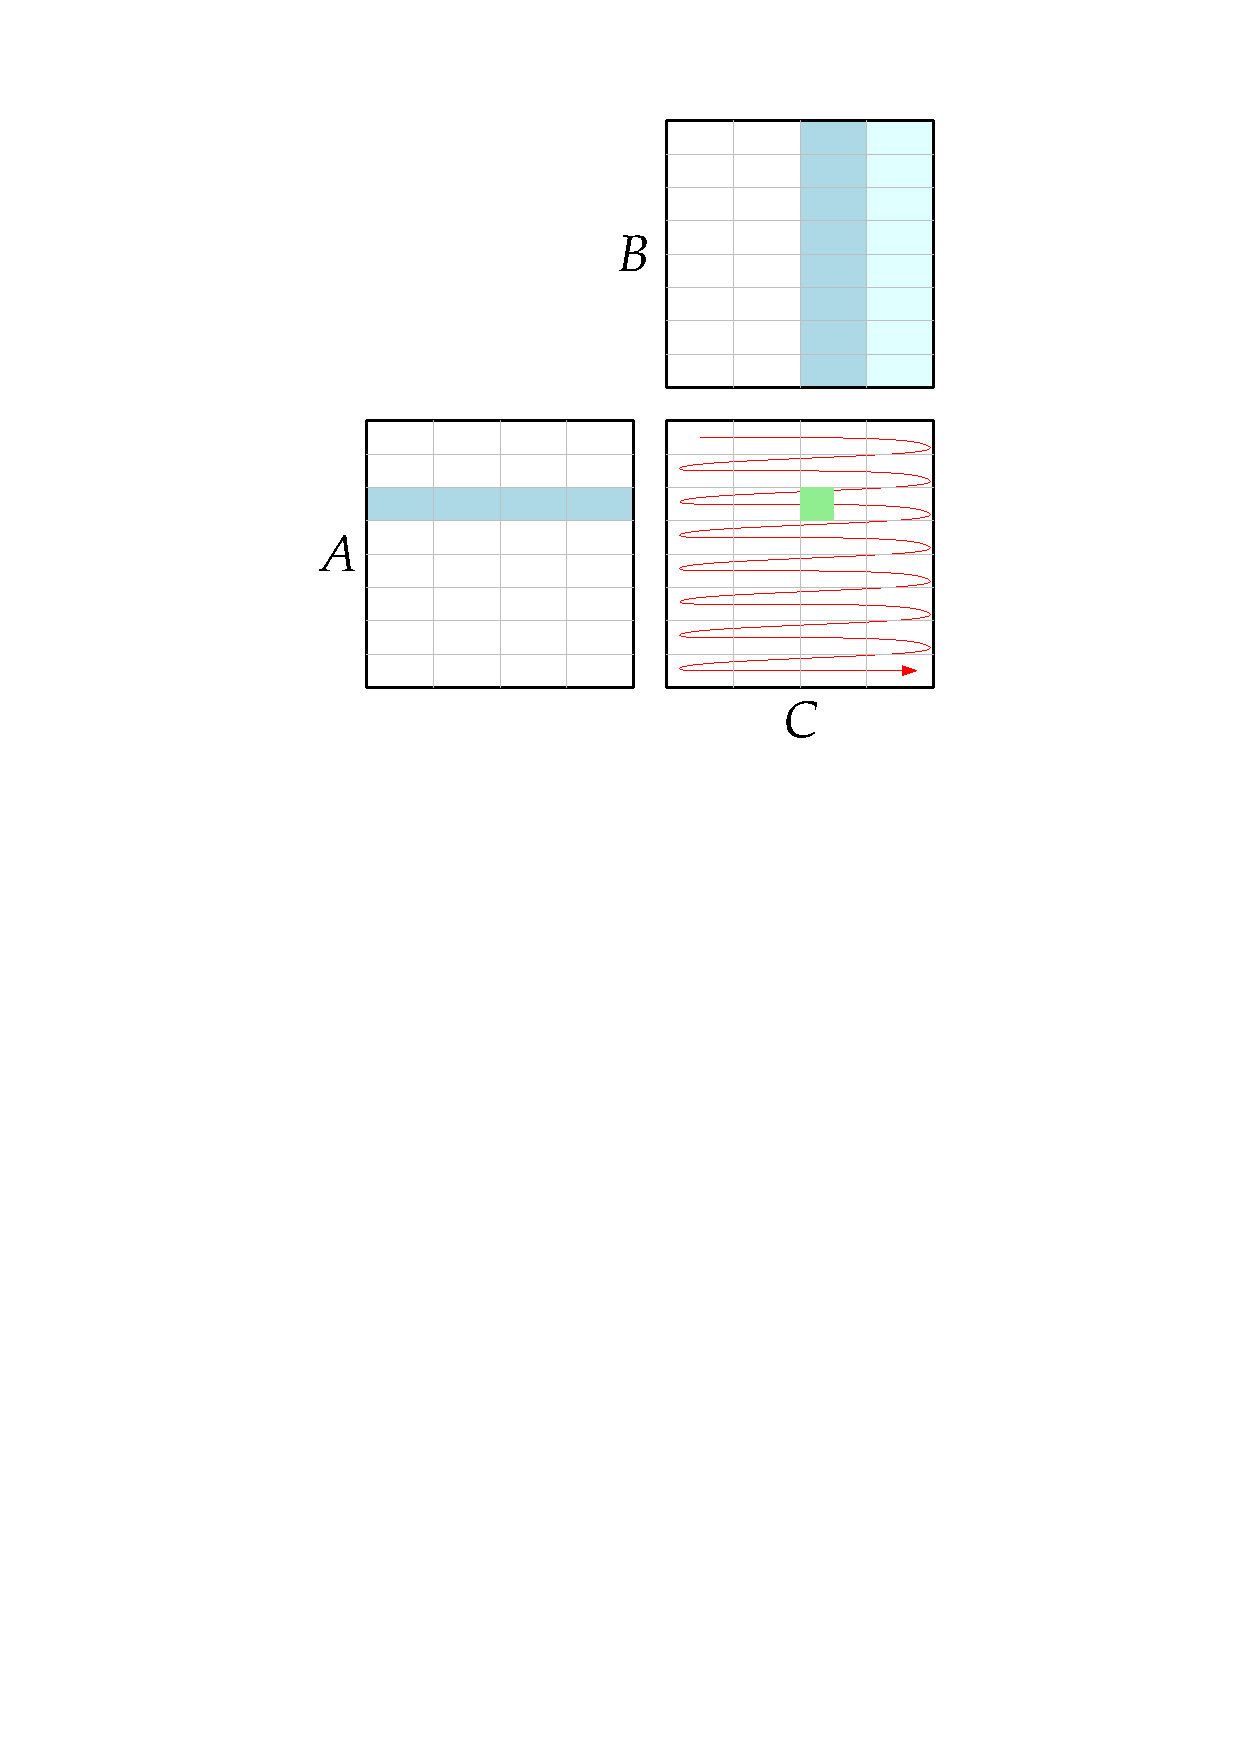
\includegraphics[width=8cm]{images/rowrowmul}
  \caption{Illustration of multiplication with row-row layout.}
  \label{fig:rowrowmul}
\end{figure}

We want to compute the matrix product $C = AB$. We do this by filling
out all entries in $C$ in a row-by-row and inside a row,
column-by-column fashion. 

If the $B$ matrix and one row of the $A$ matrix are sufficiently small
to fit into the cache, the naive matrix multiplication will only fetch
every cache line once, leading to $2n\frac{n}{B}$ cache faults. This
happens when
\[
n^2 \cdot 8 + 8n \leq \mathcal{M}
\]
For the L2 cache this limit is at $n \approx 180$, for the L3 it is $n
\approx 1023$.

If the matrices are a bit larger, then the columns of $B$ will be
evicted from the cache, but the current row of $A$ will not be
excluded. In order for this to happen, we should have enough cache to
store all the cache lines used in matrix $B$ (to fill the current
row). These are the cache lines marked with the darker blue color in
Figure~\ref{fig:rowrowmul}. Because the CPU uses an adjacent cache
line prefetcher, we also expect it to load the next cache line, hence
we also expect the area marked with light blue to be in cache. If we
let $\mathcal{M}$ denote the size of the cache in bytes, then we find
that we can reuse the cache lines of $C$ only if
\[
( n + n \cdot \underbrace{8}_{\mathclap{8 \text{ doubles in a cache line}}} \cdot 2) \cdot 8 \leq \mathcal{M}.
\implies
n \leq \frac{\mathcal{M}}{136}.
\]
Since the cache works in a LRU like fashion[citation?], we will get no
benefit from the loaded cache lines of the $B$ matrix if the cached
elements does not fit. For example, the L2 cache, which is $256kb$,
will begin to trash the values when
\[
n \leq \frac{256 \cdot 1024}{136} \approx 1927.
\]
We will analyze the expected number of cache faults in both situations.

In order to estimate the number of cache faults, we will consider the
number of cache faults incurred when computing one line in the $C$
matrix. When we begin to calculate the next line, we will not be able
to reuse any cache data, since we start computation from the first
column\footnote{We made some experiments where we tried to move
  backwards through the columns every second row. We suspected this to
  maybe improve cache performance, because we made more local
  work. However it turned out that this approach yielded a running
  time about $60\%$ slower!}. Hence, every row in $C$ produces cache
faults independently of each other.

When calculating a row, and we assume that the cache is big enough to
store the data needed, as illustrated in figure~\ref{fig:rowrowmul},
we initially get $\frac{n}{B}$ cache faults from reading a row in $A$.
Afterwards we make $n$ cache faults from loading a column in
$B$. These entries can be used for the computation of the entire cache
block of $C$, thus we will encounter $n \cdot \frac{n}{B}$ cache
faults from the $B$ matrix. Therefore we find the total number of
cache faults to be
\[
\left( \frac{n}{B} + n \frac{n}{B} \right) n = \frac{n^2}{B} \left( 1 + n \right).
\]
If the rows of $B$ does not fit the cache, we have a quiet different
situation. Then all the values of both the $A$ and $B$ matrices will
be trashed. Therefore we will for every calculation fetch a row in $A$
and all columns in $B$. This gives us
\[
n\left( \frac{n}{B} + n \right) n = n^3 \left(1 + \frac{1}{B} \right)
\]
cache faults\footnote{Notice that we does not pay for cache faults
  when writing. This is because L2 cache is not write
  allocate. TODO: CHECK THIS!}.

We do not expect any significant amount of branch mispredictions.

\subsubsection{Row/column-based layout}
In order to improve the number of cache faults, we have tried to use a
column base layout in the right operand in the multiplication. We
expect this to give us a bit better cache performance. This approach
has the drawback of limiting a matrix only to be used on one side of a
multiplication. However, this problem can be mitigated by conversions
which is an $O(n^2)$ operation.

We will give estimates of the number of cache faults occurring when
multiplying two matrices. This will be done similarly to the previous
section. The situation now looks as illustrated in
figure~\ref{rowcolmul}.
\begin{figure}[h!]
  \centering
  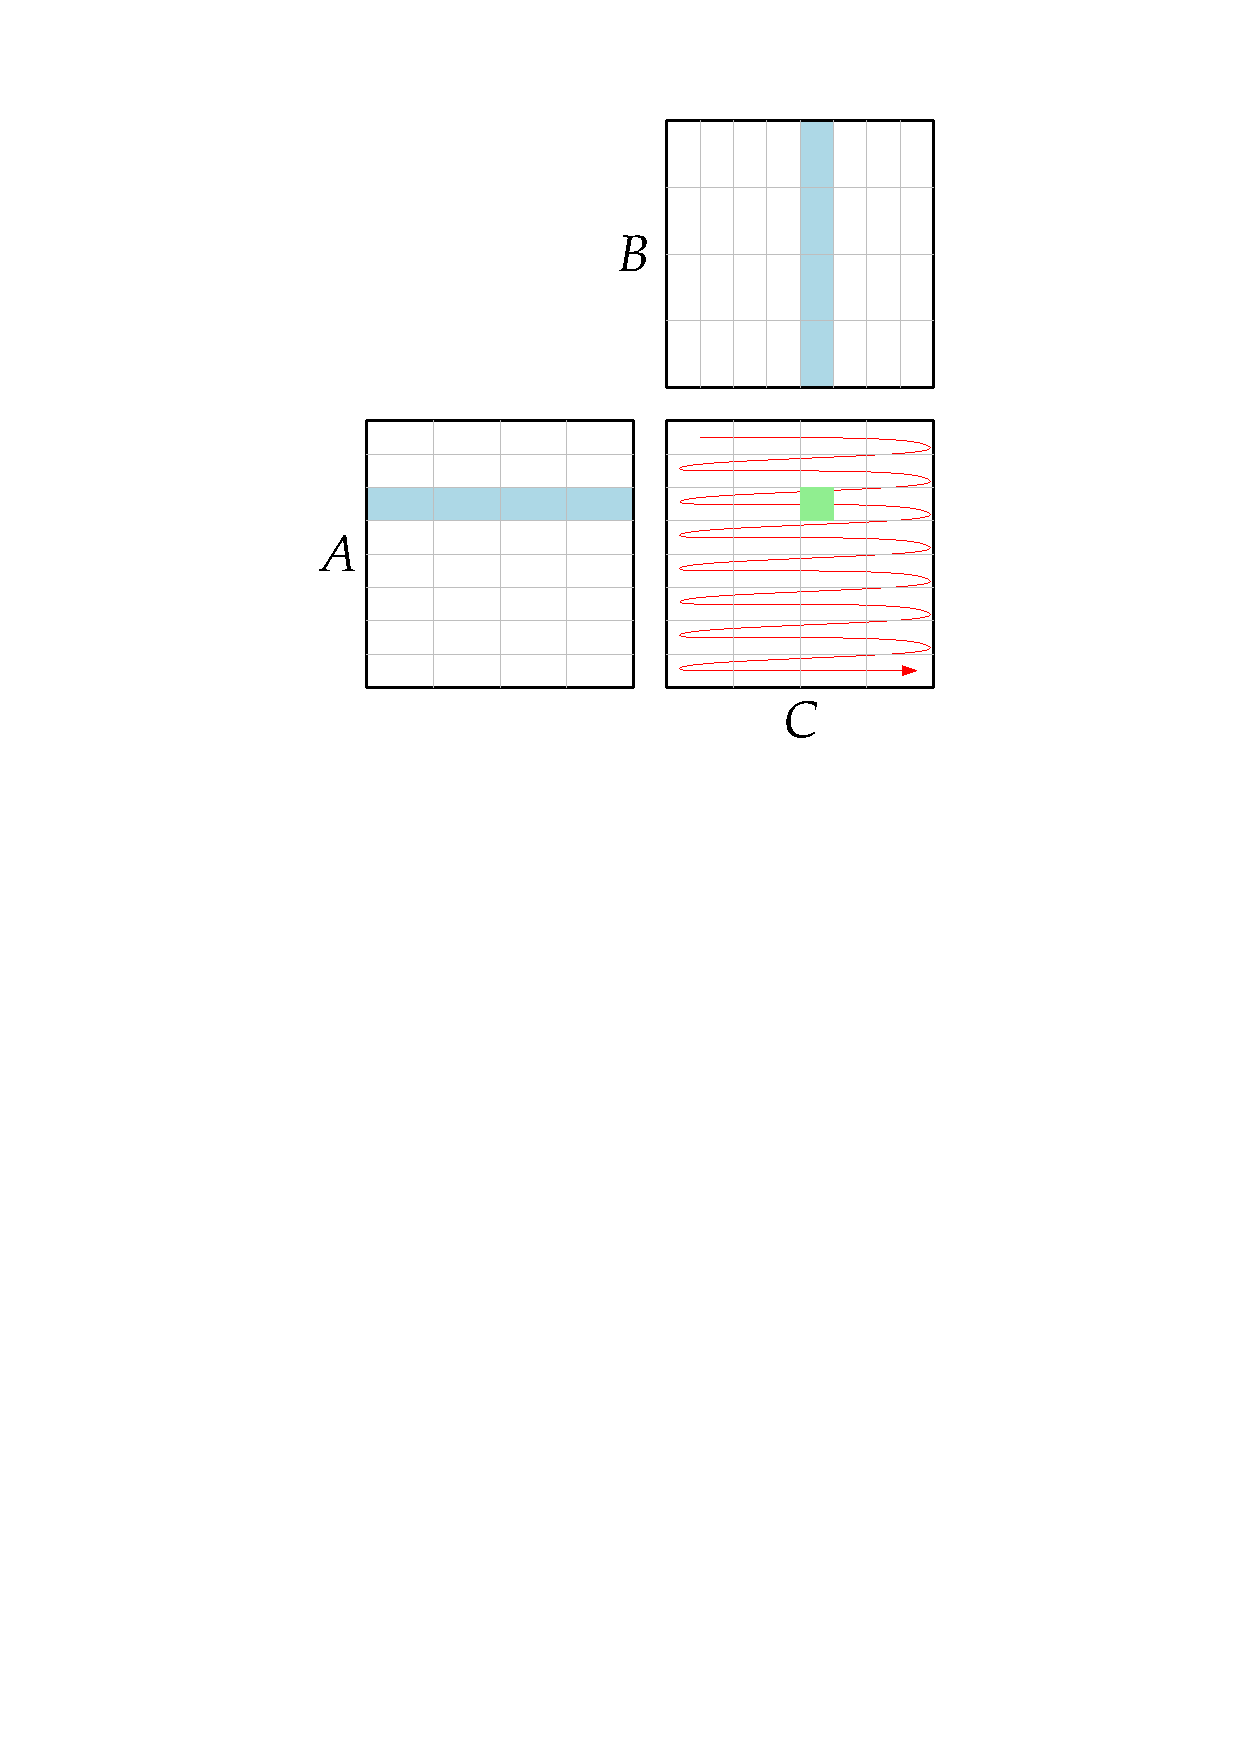
\includegraphics[width=8cm]{images/rowcolmul}
  \caption{Illustration of multiplication with row-col layout.}
  \label{fig:colowmul}
\end{figure}

First off, if the matrices are sufficiently small all entries used
fits the cache then, like in the row-row case, we get $2n\frac{n}{B}$
cache faults. This happens at the same points as in the row-row
analysis, that is for the L2 cache $n \approx 180$, and for L3 $n
\approx 1023$.

We will now estimate for what values of $n$ we can keep the current
column of $B$ in cache. This is found by
\[
(n + n)8 \leq \mathcal{M} \implies n \leq \frac{\mathcal{M}}{16}
\]
For the L2 cache with $\mathcal{M} = 256kb$ we find that
\[
n \leq \frac{256 \cdot 1024}{16} = 16384.
\]
That is, a number that is much larger than any of our test instances
(when using a row-column based layout). We will therefore focus on the
analysis where a column of $B$ actually fits the cache. We will again
do the analysis for one row in $C$, and then, since the next row does
not share any cache data with the previous (except if the matrices are
really small), we can multiply the number of cache faults for each
row. We first get $\frac{n}{B}$ cache faults from matrix $A$. Then we
get $\frac{n}{B}$ cache fault from a column in $B$, which we do for
each of the $n$ columns, giving a total of
\[
\left( \frac{n}{B} + n \frac{n}{B} \right) = \frac{n^2}{B}\left(1 + n \right)
\]
cache faults. This is exactly the same number of expected cache faults
as in the row-row layout, when that is also in the good case.

When we can not hold the column of matrix $B$ in cache, we expect
\[
\left( \frac{n}{B} + \frac{n}{B} \right) n^2 = \frac{2n^3}{B}
\]
cache faults. This number is better than in the row-row case, and it
should begin to show much later then the row-row layout.

\subsection{Recursive multiplication}

For exploiting more kinds of layouts we implemented the recursive algorithm.

\subsubsection{Z-curve layout}

The first idea was to use a Z-curved layout. One major advantage of this layout is that improves locality on all levels of the recursive multiplication. The drawback is that the index calculations are time consuming. On x86 we get approximately 50 bitwise operations each time we want to convert a coordinate to the position in the array. However, this can be improved by incrementally constructing the Z-curve numbers or by precomputing offsets at base cases. The upcoming Intel Haswell architecture has support for bit permutations which will improve the situation.

We ended up with precomputing the Z-curve offsets at the base case. That means the only penalty when we want to store or lookup a value is a level of indirection. In the recursive algorithm we used 8*8 as a base case for switching to the naive algorithm.

\subsubsection{Tiled layout}

A tiled layout is a compromise between locality and performance of index calculations. When the recursive algorithm reaches blocks of the same size as the tiles, it switches to the naive algorithm. And the naive algorithm functions without any modifications. To improve cache locality a bit we used a row-based layout in the tiles for the left operand and a column-based layout in the tiles for the right operand.

We also tried an iterative algorithm with a tiled layout. But it did not perform well compared to the recursive due to cache locality so we decided to omit it.

$\Theta(n+n^2/B + n^3/B\sqrt{\mathcal{M}})$
\todo{Her er formelen fra artikel omkring cache faults}

\subsection{Strassen}

Strassen exploits some tricks with matrix multiplication such that it only uses 7 multiplications instead of 8 multiplications. It is a recursive algorithm by nature. The first step of the algorithm is to split the operands into 2*2 blocked matrix.

Instead of actually splitting the matrix into smaller matrices we have used a Z-curve layout. That means that the smaller matrices are able to just point to the data in the parent matrix (instead of actually copying) while still preserving a proper layout themselves.

Strassen needs to have a large base case such that we do not spend too much time on the recursion and to improve cache locality at the base levels. 32*32 seemed to be a good choice on our platform. To avoid the overhead of handling matrix multiplication with a level of indirection or by calculating Z-curve indices, we used a row-based and column-based layout at the base case for the left and right operand respectively.

The additions and subtractions in the algorithm only works on left operand block matrices or right operand block matrices. Therefore, we can use a single loop and no index calculations to add and subtract matrices. I.e. Z-curve indices are the same and we only add/subtract row-based base cases with row-based base cases etc.

One major drawback of the algorithm is that we have to allocate 7 temporary matrices of one fourth of the size of the resulting matrix + at least one extra used by the calculation of the temporary matrices. Therefore, a two input matrices of size 1024 * 1024 containing double precision floating points needs ~5*8 MB instead of 3*8 MB. Additionally, the algorithm assumes that the input matrix sizes are power of two which can lead to 4 times more memory usage if padding is employed. By using padding at each level less memory is used but it is slightly slower to pad/unpad multiple times.

One improvement we have made to the algorithm is to allocate all the temporary matrices in a stack-like fashion such that we reduce the number of cache evictions when we start writing at new locations instead of reusing locations already in cache.

Furthermore, the algorithm does lend itself to more numerical instability as described in \[strassen_stability.pdf\].\todo{citation}

According to \[ ref til matrix paper \] we should expect $\Theta(n+n^2/B + n^{\log 7}/B\mathcal{M}^{(\log 7)/2-1})$ cache faults assuming that the cache is tall ($\mathcal{M} = \Omega(B^2)$) which is true for our test CPU. Therefore, the algorithm is expected to perform fewer instructions and have fewer cache faults than the regular recursive algorithm.

\subsection{SIMD instructions}

We extended some of the algorithms with SIMD instructions from Intel Advanced Vector Extensions (AVX). Specifically we changed the naive and base cases for the recursive and Strassen which uses the naive algorithm.

For computing a cell in a matrix we exchanged the dot product loop such that it read, multiplied, and added four values each time. We also added AVX instructions for matrix additions and substractions for Strassen.

Our expectations are that the performance will increase while cache faults should be stable because we still need the same data. 

\subsection{Parallelization}

This subsection describes how we parallized some of the previously mentioned algorithms. One disadvantage when parallizing is that the L3 cache is effectively splitted into the number of cores if the threads work on independently data. An advantage, however, is that we get more L1 and L2 cache available in total.

\todo{SIMD giver ikke ligesaa meget naar parallelet. Maaske giver hyper-threading ikke ligesaa meget}

\subsubsection{Row/column-based layout}

The naive algorithm which is used for this combined is easily parallelizable because we can assign intervals of rows for each thread. The result matrix is stored in a row-based layout so writing is separated such that cache thrashing should not be a problem.

\subsubsection{Strassen}

Strassen was parallelized by starting new threads at each of the 7 multiplications. This was done at 1 or 2 levels depending on the level of parallization we wanted. The last additions/subtractions and combine operations were not parallelized. However, the multiplications uses most of the time.

One problem Strassen has compared to other algorithms is that it allocates temporary matrices. This problem gets more severe with parallization because now each thread allocates temporary matrices and therefore the memory consumption is higher than the sequential version.

Another problem we faced was that our custom stack-like allocator was not thread-safe so it is disabled for parallization. A simple lock-based approach yielded too much congestion. One suggestion to improve this is to give each thread their own allocator.
